%%
%% This is file `sample-acmsmall-tagged.tex',
%% generated with the docstrip utility.
%%
%% The original source files were:
%%
%% samples.dtx  (with options: `all,journal,acmsmall,tagged')
%% 
%% IMPORTANT NOTICE:
%% 
%% For the copyright see the source file.
%% 
%% Any modified versions of this file must be renamed
%% with new filenames distinct from sample-acmsmall-tagged.tex.
%% 
%% For distribution of the original source see the terms
%% for copying and modification in the file samples.dtx.
%% 
%% This generated file may be distributed as long as the
%% original source files, as listed above, are part of the
%% same distribution. (The sources need not necessarily be
%% in the same archive or directory.)
%%
%%
%% Commands for TeXCount
%TC:macro \cite [option:text,text]
%TC:macro \citep [option:text,text]
%TC:macro \citet [option:text,text]
%TC:envir table 0 1
%TC:envir table* 0 1
%TC:envir tabular [ignore] word
%TC:envir displaymath 0 word
%TC:envir math 0 word
%TC:envir comment 0 0
%%
%% The tagged file should start with the metadata commands.
%% We also need currently use lualatex-dev for compilation!
%% The first command in your LaTeX source must be the \documentclass
%% command.
%%
%% For submission and review of your manuscript please change the
%% command to \documentclass[manuscript, screen, review]{acmart}.
%%
%% When submitting camera ready or to TAPS, please change the command
%% to \documentclass[sigconf]{acmart} or whichever template is required
%% for your publication.
%%
%%
\documentclass[sigchi]{acmart}
%%
%% \BibTeX command to typeset BibTeX logo in the docs
\AtBeginDocument{%
  \providecommand\BibTeX{{%
    Bib\TeX}}}

%% Rights management information.  This information is sent to you
%% when you complete the rights form.  These commands have SAMPLE
%% values in them; it is your responsibility as an author to replace
%% the commands and values with those provided to you when you
%% complete the rights form.
\setcopyright{acmlicensed}
\copyrightyear{2018}
\acmYear{2018}
\acmDOI{XXXXXXX.XXXXXXX}

%%
%% These commands are for a JOURNAL article.
\acmJournal{JACM}
\acmVolume{37}
\acmNumber{4}
\acmArticle{111}
\acmMonth{8}

%%
%% Submission ID.
%% Use this when submitting an article to a sponsored event. You'll
%% receive a unique submission ID from the organizers
%% of the event, and this ID should be used as the parameter to this command.
%%\acmSubmissionID{123-A56-BU3}

%%
%% For managing citations, it is recommended to use bibliography
%% files in BibTeX format.
%%
%% You can then either use BibTeX with the ACM-Reference-Format style,
%% or BibLaTeX with the acmnumeric or acmauthoryear sytles, that include
%% support for advanced citation of software artefact from the
%% biblatex-software package, also separately available on CTAN.
%%
%% Look at the sample-*-biblatex.tex files for templates showcasing
%% the biblatex styles.
%%

%% use of package for code snippets
\usepackage{tabularx}
\usepackage{subcaption}
\usepackage{float}
\usepackage{multirow}
\usepackage{array}
\usepackage[dvipsnames]{xcolor}

%%
%% end of the preamble, start of the body of the document source.
\begin{document}

%%
%% The "title" command has an optional parameter,
%% allowing the author to define a "short title" to be used in page headers.
\title{Investigating Management and Attention towards Household Appliances During Cooking}

%%
%% The "author" command and its associated commands are used to define
%% the authors and their affiliations.
%% Of note is the shared affiliation of the first two authors, and the
%% "authornote" and "authornotemark" commands
%% used to denote shared contribution to the research.
\author{Lah Hong Wai}
\affiliation{%
	\institution{Bauhaus-Universität Weimar}
	\city{Weimar}
	\country{Germany}}
\email{lah.hong.wai@uni-weimar.de}

\author{Daniel Radianto}
\affiliation{%
	\institution{Bauhaus-Universität Weimar}
	\city{Weimar}
	\country{Germany}}
\email{daniel.cristianindra.radianto@uni-weimar.de}

\author{Xavier Theodosius}
\affiliation{%
	\institution{Bauhaus-Universität Weimar}
	\city{Weimar}
	\country{Germany}}
\email{xavier.julian.theodosius@uni-weimar.de}


%%
%% By default, the full list of authors will be used in the page
%% headers. Often, this list is too long, and will overlap
%% other information printed in the page headers. This command allows
%% the author to define a more concise list
%% of authors' names for this purpose.
\renewcommand{\shortauthors}{Lah et al.}

%%
%% The abstract is a short summary of the work to be presented in the
%% article.
\begin{abstract}
	Cooking is a complex activity that requires people to coordinate multiple appliances while managing time, safety, and task demands in their personal space. Understanding how attention is distributed during cooking is important for Human-Computer Interaction, as breakdowns in attention can lead to errors or unsafe situations. Using remote re-enactment video as a method, this study investigates how individuals distribute attention and interaction across kitchen appliances during cooking. Despite limitations such as a restricted field of view and limited contextual information, the collected data allowed observation of cooking sequences, attention shifts, and task transitions. Qualitative thematic analysis revealed recurring patterns in how participants coordinated actions, managed timing, and maintained situational awareness while cooking. The findings highlight that attention management relies on continuous adjustment rather than constant focus, and indicate that both timing and situational awareness play important roles in shaping the cooking workflow, as multiple tasks are carried out in parallel and often depend on one another. Collectively, cooking heavily emphasizes maintaining a workflow through continuous shifts in attention and interaction across appliances.
\end{abstract}

%%
%% The code below is generated by the tool at http://dl.acm.org/ccs.cfm.
%% Please copy and paste the code instead of the example below.
%%
\begin{CCSXML}
	<ccs2012>
	<concept>
	<concept_id>10003120.10003121</concept_id>
	<concept_desc>Human-centered computing~Human computer interaction (HCI)</concept_desc>
	<concept_significance>500</concept_significance>
	</concept>
	<concept>
	<concept_id>10003120.10003121.10011748</concept_id>
	<concept_desc>Human-centered computing~Empirical studies in HCI</concept_desc>
	<concept_significance>300</concept_significance>
	</concept>
	<concept>
	<concept_id>10003120.10003121.10003122.10003334</concept_id>
	<concept_desc>Human-centered computing~User studies</concept_desc>
	<concept_significance>300</concept_significance>
	</concept>
	<concept>
	<concept_id>10003120.10003138</concept_id>
	<concept_desc>Human-centered computing~Ubiquitous and mobile computing</concept_desc>
	<concept_significance>100</concept_significance>
	</concept>
	<concept>
	<concept_id>10003120.10003121.10003128</concept_id>
	<concept_desc>Human-centered computing~Interaction techniques</concept_desc>
	<concept_significance>100</concept_significance>
	</concept>
	</ccs2012>
\end{CCSXML}

\ccsdesc[500]{Human-centered computing~Human computer interaction (HCI)}
\ccsdesc[300]{Human-centered computing~Empirical studies in HCI}
\ccsdesc[300]{Human-centered computing~User studies}
\ccsdesc[100]{Human-centered computing~Ubiquitous and mobile computing}
\ccsdesc[100]{Human-centered computing~Interaction techniques}

%%
%% Keywords. The author(s) should pick words that accurately describe
%% the work being presented. Separate the keywords with commas.
\keywords{Cooking behavior, Attention, Interaction, Re-enaction Video, Remote Studies, Qualitative Analysis}

%%
%% This command processes the author and affiliation and title
%% information and builds the first part of the formatted document.
\maketitle

\section{Introduction}

 Cooking is an integral activity in daily life. A combination of appliances can be used for this activity, including sanitization, food preparation, and serving. Using kitchen appliances during cooking requires a certain level of attention. Although cooking does not require constant focus, interruptions or shifts in attention can lead to mistakes or safety issues if the ongoing cooking process is forgotten. Maintaining awareness of active appliances, particularly those that involve heat or sharp objects, is therefore important during cooking. Without proper attention while cooking, accidents such as burnt food, overheated utensils, and even accidental harm can occur due to minor distractions or inattention. Understanding how attention and interaction work during cooking is crucial for Human-Computer Interaction, as cooking is a complex, real-world activity that combines physical actions, cognitive decision-making, and time management. By examining cooking as an everyday practice, this research aims to understand how people naturally manage multiple technologies in their home environment.
  
 This study focuses on how each individual distributes their attention and interacts with appliances. Attention is understood as the mental focus at a given time, while interaction is more about how an individual can create engagement across appliances, such as cleaning, preparing a serving place, or responding to alerts. Rather than treating appliance use as isolated actions, this research views cooking as a dynamic process in which users continuously adjust their focus in response to task demands, the appliance's response, and the current situation. Investigating these patterns can reveal how people prioritize tasks, manage interruptions, and coordinate actions across devices.   
  
 Building on this perspective, the research question guiding this study is: “How do individuals distribute attention and interaction across household appliances during everyday cooking?” This is an exploratory qualitative study that does not aim to establish causal relationships, but to identify recurring patterns of attention distribution and interaction. Using re-enactment video as the chosen qualitative method, the study seeks to understand how attention shifts across appliances and what factors influence these shifts, such as task importance, timing, and perceived risks (e.g., burning food or overcooking). Interactions are expected to concentrate around specific moments, including preparation, monitoring progress, and responding to changes during the cooking process.

\section{Methodology}

Studying how individuals distribute attention across different household appliances during everyday cooking presents challenges, as attention shifts and coordination are difficult to capture in real time. Prior research addressed these challenges by employing re-enacted scenarios to capture interaction and routines \cite{Pink2017Design}. Drawing on insights from previous studies \cite{Buchenau2000}, the present study adopts re-enactment videos (REV), where they capture individuals re-enact a particular scenario from their everyday cooking. Video re-enactment was selected as it was an appropriate method to explore and understand participants' experiences, visible and hidden \cite{Pink2015DoingSensoryEthnography}. Themes were then developed through thematic analysis from the data.

To undertake this research, we focused on understanding how interaction was done with household appliances during cooking, and how attention could be distributed. Particular attention was paid to transitions between commonly used kitchen appliances, such as the refrigerator, stove and sink, which are commonly described as a ``kitchen work triangle''. This concept was only used as a guide to prioritise observation of kitchen appliances, and was not involved in the analytical framework. To adopt this method, we used visual techniques to record the actions, followed by a post-interview review of the recorded videos. During the re-enactment, participants were encouraged to think-aloud, to better understand their actions.

Prior to the main study, a pilot session was conducted to understand the re-enactment flow, video setup and prompting strategy. This session led to minor refinements to the study, including reducing prompting to avoid interruption and finding good angles for recording. Data from the pilot session were not included in the final analysis.

\subsection{Participants}

Recruited participants were initially screened to ensure they had prior experience with everyday home cooking and familiarity with using common household appliances. Three participants took part in the study, ranging in age from 24 to 30 years. Participants were recruited via convenience sampling, based on availability and willingness to take part in the study.

All participants reported cooking at home several times per week. They were all familiar with commonly used kitchen appliances, including a stove, refrigerator, and sink. One participant mentioned cooking for oneself, particularly for meal prep. Another participant reported a shift from cooking for household to only one due to a change in living situation. Cooking for household as a responsibility was noted for the third participant. Participants selected dishes with varying complexity. The dishes chosen were stir-fry with vegetables and minced meat, meal-prep with chicken and dish involving lentils.

This study involved a small number of participants (N = 3) and was conducted in a domestic setting. This was done to focus on gaining in-depth insights in the experiences of individuals, on how attention and interaction are distributed across household appliances during everyday cooking, rather than statistical results.

\subsection{Materials}

Due to the nature of this study, participants were only required to perform re-enactments in their domestic kitchen environment. All participants provided consent prior to the participation. Only a recording device was required by the participant to capture interaction. No specialised equipment was provided to participants for the study. Data were collected remotely using Google Meet, which was used to record video and audio of cooking activities and participant commentary.

Recordings were transcribed using Condens.io to support qualitative analysis. Data were stored securely in a device accessible only to the researchers. To illustrate and pick key interaction sequences to supplement the analysis, video recordings were translated into participant-specific storyboards.

\subsection{Procedure}

During the screening session, participants were requested to select a recipe that they were comfortable with. In the re-enactment, they were asked to perform a cooking scenario based on the recipe. They were allowed to select a time context (e.g. lunch, dinner) which they find suitable for their selected recipe. Little guidance was given, besides giving them examples of the starting and ending point of a cooking process. We allowed these points to be freely selected by the participants, such that we could capture any insightful scenarios that may not be part of a cooking process such as cleaning up after dinner. These scenarios could help explain participant-specific interaction patterns observed during cooking.

This re-enactment was facilitated by one researcher, where limited prompts were given during the session for further understanding. The prompts were asked in each ``break'' \textemdash~ short sessions where participants transitioned from one sub-action to another, such as chopping to cooking \textemdash~ to ensure the process remains uninterrupted. While re-enacting, participants were encouraged to narrate on their interactions. They were also told that they should not reveal, say or answer anything that were felt uncomfortable. After this session, the researchers re-watched the video, noting down important actions and interactions that require more explanation. Another session, but not recorded, was done with the participants to assist in understanding the peculiar parts, supported by the recorded video.

\subsection{Spatial Context of Cooking Activities}

To complement the discussion of spatial movement and appliance coordination during the cooking activities, one participant consented to showing the kitchen floor plan. Therefore, a simplified schematic floor plan of the kitchen was drawn, shown in Figure~\ref{fig:context_1}. The floor plan illustrated only the main appliances that the participant often interact with. Exact dimensions of the kitchen layout were not recorded, as we only wanted to understand relative spatial relationships between appliances rather than precise measurements.

\begin{figure}[H]
	\centering
	\includegraphics[width=\columnwidth]{figures/p1_plan.png}
	\caption{\textbf{Schematic floor plan of the kitchen.} These dimensions were not representative of the owner's actual dimension.}
	\label{fig:context_1}
\end{figure}

Further understanding of the interaction with the stove was needed to support the interpretation of participants' interaction. This presented as a useful aid to actions that the video could not capture, due to viewing area limitations. The same participant also consented to the inclusion of a schematic sketch of the stove interface, shown in Figure~\ref{fig:context_2}.

\begin{figure}[H]
	\centering
	\includegraphics[width=\columnwidth]{figures/p1_cook.png}
	\caption{Schematic of the stove.}
	\label{fig:context_2}
\end{figure}

The stove contained two induction hobs, operated through electricity. The hob is turned on by holding the power button (placed at the right of +) for 2 seconds. The temperature is adjusted with the increase + and decrease - buttons around the display, located between the two buttons. The most left button was a child lock button, to prevent children from accidentally switching on the stove.

These two figures will be used to complement findings that require more elaboration and challenges that the participant had faced.

\subsection{Data Analysis}

Recordings and transcripts were stored in a cloud folder with password protection, and only shared among researchers involved in this study. These materials were used for thematic analysis \cite{BraunClarke2021}, where we identify recurring patterns to understand underlying meanings of participants in their cooking re-enactment. The transcripts were analysed for interesting quotes, retrieved and then placed in Figma for collaboration. 

We went through a five-stage process, with iteration when appropriate, following Braun and Clarke's guidance \cite{BraunClarke2021}. Each interesting quote was designated a code in the first cycle. The second stage involved refining codes, discarding duplicates and removing superfluous quotes. Patterns were found among codes, grouped and themes were later identified.

In addition, the videos were also analysed. Actions involving hands, routes, activities, materials used, senses and cues were recorded. Facial expression was also scrutinised when participants encountered challenges. To facilitate the understanding of relationships between actions and narrations, transcripts were viewed alongside with videos, and actions noted down. Separating these two presents a false construct because the narration may not accurately reflect the actions, frequently done unintentionally or not knowingly, and interesting insights may be omitted. Therefore, both resources were used together for the analysis.

\section{Findings}

In this section, we report our themes supported by quotes and interactions from videos, in which people direct attention as a dynamic resource towards senses, risks, coordination and spatial management. We describe results that were either obvious or unexpected from the re-enactment sessions and think-aloud activity, to complement the themes that we had constructed.

\subsection{Theme 1: Coordinating Attention Across Multiple Appliances}

This theme captures how participants distribute attention and interaction across multiple appliances during cooking. The observations under this theme focus on the actions of the participants and how they decide the priority of each appliance, illustrating how participants coordinated actions, shifted attention, and responded to ongoing task demands.

\subsubsection{Subtheme: Sequential and Parallel Appliance Use}

Participants were observed switching between using one appliance only or multiple appliances to coordinate cooking activities. Certain actions required a strict sequence to achieve their desired outcomes. One participant mentioned that cooking garlic was imperative to proceed to the next step: ``Of course, the garlic must be fried first.''

Appliances and tools were also frequently used together to maintain workflow efficiency. While food was cooking on the stove, participants engaged in other tasks rather than waiting for the food to be done. `I am going to put the rest of the chicken in the fridge.'', as the primary cooking task simmered in the pot.

Observations revealed that participants were actively organising their workspace during cooking to support their parallel tasks. For example, the sink had limited space, therefore dishes that remained must be washed and left in the dryer before another set of dirty dishes could be placed inside. These actions enabled them to maintain task flow and reduce interruptions.

\subsubsection{Subtheme: Unintentionally Delaying Actions Until Conditions Are Met}

Not every workflow was always smooth, as participants partake in decision making when selecting appliance and tools. It was observed that they delayed actions intentionally due to missing conditions, or a task required higher priority. While not necessarily a smooth workflow, these actions sometimes carried a reason. ``The spatula I will put it into wok, maybe I'll still need afterwards'', as the washing of the spatula was postponed.


It was often seen at times that the delay can also be caused by a difficulty in estimating the right kitchen tool sizes. While it was expected that it will be challenging to select a right size, participants can be seen deciding on a size that was ``big enough''. This decision helped to avoid problems of inadequate fit and subsequently allowed commencing other tasks. What was unexpected, was that they may take a longer time to decide what ``big enough'' meant, often changing plate or bowl sizes to find one suitable. Nonetheless, this was not a deterrent to their workflow, as a smooth transition to the next task was observed.

\subsubsection{Subtheme: Managing Unintended Delays caused by Safety or Space Constraints}

Delays were also caused by space constraints or safety features. This delay resulted in more noticeable disruption, requiring participants to adjust the sequencing of subsequent actions. It was also more disruptive in that the actions cannot be postponed, and must be resolved for the intended flow \textemdash~the main cooking task\textemdash~to continue.

Delays by safety constraints was more frequently shown by participants who utilised electric variants of appliances, such as an induction hob. One participant's stove had a safety feature integrated to prevent children from accidentally switching it on, known as child-lock, as shown in Figure~\ref{fig:context_2}. However, there was once where it was unintentionally activated, which disabled every other button's functionality. Visible frustration could be seen from the participant as the child-lock button must be held for 2 seconds to enable stove functionality again. Although the participant did not comment, the design of this induction hob was unfavourable and interrupted the cooking process.

Space constraints were less disruptive to the safety counterpart. From the quick actions and decision-making, it was noted that participants acknowledged the problems with space, and had a solution ready to prevent further interruption. One participant had lack of counter space, but required space to place bowls. Re-arrangement was needed to fit the bowl, and in one observed case, the participant placed the bowl with the least priority in the current process at a further place to make space for other bowls.

\subsection{Theme 2: Applying Knowledge, Experience and Strategies to Maintain Control}

This theme focuses how participants applied current knowledge, experience and strategies to control the cooking process. This will be complemented by observations on reasons explicitly stated by participants on certain actions for a precise outcome.

\subsubsection{Subtheme: Switching between Experience-Based Judgment and Precise Measurements}

Participants often alternated between thinking and applying measurement tools when interacting with kitchen appliances and tools. They preferred using experience when the process did not require fine measurements or presented a possibility to be corrected later, such as adding salt during taste-testing: ``I would try whether is adequate enough or needs more seasoning''. These decisions were done quickly with minimal visual confirmation, which enabled attention to be distributed to other tasks. 

Precise measurement was required in situations that were less familiar or was mandatory for a desired outcome. Examples were carefully measuring quantities or ensuring temperature was adequate. In these situations, it was observed that there were lesser parallel activity, limited to ensure accuracy. A participant required that his ingredient was precisely measured, stating that ``I’m going to take my weighing scale''.

Transitions occurred dynamically during cooking, where shifts were done according to demand changes, such as approaching critical stages during the cooking process. The observations indicated that attention was constantly adjusted according to the task sensitivity, helping participants to achieve their desired outcomes.

\subsubsection{Subtheme: Preparing Components In Advance to Reduce Errors}

A common observation was noted in that every participant participated in an `ingredient-preparatory' phase, where the ingredients must be taken out and prepared before moving on to cooking. Later it was shown that this had helped greatly with the efficiency of cooking, as the required components were positioned close to the main appliances, such as chopped vegetables near the wok.

Participants were requested to select a starting point for what they thought was cooking. Every participant started with a storage, whether it was a refrigerator or a drawer. They began gathering the items required for their dish, and placed them in proximity (often next to) to the stove. nce cooking was underway, participants relied on the prepared components to proceed with fewer interruptions, with attention focused on monitoring and timing.

This preparation phase was also seen to have eliminated frequent movements in relation to spatial context. Figure~\ref{fig:context_1} illustrated one participant's floor plan, where the fridge was positioned a distance away from the area where most actions took place. During the session, the participant had not moved towards the dry kitchen except for when cooking was done. Therefore, preparing ingredients in advance helped in reducing frequency of diverting attention to other appliances, especially when they were positioned far.

The preparatory behaviours were observed as part of an ongoing effort to maintain workflow. Participants preferred organised components, to minimise errors and then reacting to them. This showed that preparation was an important strategy to maintain attention within everyday cooking practices.

\subsection{Theme 3: Monitoring Progress through Senses and Evaluation}

Participants combined sensory cues and assessment towards their culinary to attain desired outcomes. Observations showed that attention distribution frequently occurred, in which participants used senses to check changes in food state or tools, whether they were performing secondary tasks or attentively watching the main process.

\subsubsection{Subtheme: Uses Sensory Cues to Determine Food Quality}

It was expected that participants would use senses as a guidance to actions. Varieties of sensory cues were employed and seen constantly used to evaluate outcomes. They also allowed participants to remain aware of appliance activity while performing tasks away from the immediate cooking area.

Participants either use one type of senses, or multiple simultaneously depending on the demands of the situations. They were utilised at specific moments such as approaching a completion point or a change in cooking state. One participant observed the state of the pot by ``see[ing] bubbles if the pressure is leaking''. This illustrates how sensory monitoring and evaluation supported dynamic attention allocation throughout the cooking process.

\subsubsection{Subtheme: Reflecting on Outcomes to Judge Success or Quality}

Combining sensory cues and assessment was a common occurrence to evaluate the quality of their dishes. Evaluation was based on observable qualities including appearance, texture, and perceived completion, often accompanied by brief pauses in the activity.

One monitored the garlic to ``make sure they are in like brownish colour and with an aroma smell'', which was presented as a cue to move forward to the next step. Therefore, these assessments were used to dictate completion of a step, distributing attention to the next. When results were aligned with expectations, participants proceeded without adjustment. However, when they were not desirable, they performed corrective actions, such as adjusting heat levels or revisiting earlier steps.

Evaluations were incorporated as part of the process rather than being treated as separated events. These enabled participants to regulate workflow and maintain control over cooking progress. Therefore, this highlights that assessment was integral, and that attention complements as a guidance to interaction choices across appliances. 

\subsection{Theme 4: Managing Risks and Hygiene During or Outside of Interaction}

This theme explores the importance of managing risks and hygiene during the cooking process. Participants maintained these criteria to an extent, and the significance of how each participant perceived was surprisingly varied.

\subsubsection{Hygiene Focus with Appliance, Food and Self}

Each participant perceived the important of hygiene differently. One actively stressed the importance of it, with the word ``wash'' being mentioned many times (The count for wash, washed and washing in the transcript processed was 54 times). Another decided that cleaning somewhat important, with ``I'm not going to wash my hands, nevermind, just a little sprinkle of water.''. The use of the tap and sink was therefore dependent on the individual, and attention towards cleanliness followed.

We identified three categories where hygiene was crucial: on appliances, on food and for the participants themselves. Cleaning occurred predominantly after cooking was completed, but there were also moments during cooking where waiting was required, and that was used to clean. Appliances cleaning, such as wiping the stove, occurred after cooking, because it required constant use during cooking. Food hygiene was observed more during the preparatory phase, where vegetables have to be washed or soaked. Hygiene on self happened throughout the process.

The sink was therefore mandatory, as it assisted keeping hygiene, and integral in cooking. Attention towards the sink was distributed based on demands and criteria, and participants used this to streamline their cooking process and ensure their working space could eventually be clean.

\subsubsection{Appliance Selection Based on Perceived Risk}

Participants selected appliances that were perceived as low-risk for cooking. This did not occur during the cooking, but rather when purchasing them. One participant highlighted that induction hob was preferred because ``it was safer than the gas option''. This implied that a suitable appliance was mandatory even outside of cooking, and helped shape the necessary attention to monitor and manage them.

During interaction however, participants utilised what they needed, and observations did not show that they had a preference for a safer alternative, such as using a knife of lesser sharpness. Rather, great attention was given when handling dangerous tools or operating risky appliances. This showed that during interaction, participants did not select tools based on the risk, but rather their needs.

\section{Discussion}
The results of this study suggest that attention during cooking is not a static but a dynamic, distributed resource that is directed towards sensory feedback, risk mitigation, and spatial management.

The findings in sensory cues usage suggests that individuals distribute their attention towards multiple sensory channels. Rather than constantly staring at an appliance, individuals utilized auditory (sizzling sounds) and tactile (gauging pan temperature with hands) cues. This suggests that attention is highly multimodal, as individuals 'listen' and 'feel' for progress rather than just 'seeing'. 

Furthermore, the findings also suggest that the switching between "experience-based judgement" and "precise measurement" may happen due to the attention shifts based on the perceived risk and familiarity of the task. Individuals were observed to narrow their attention towards precision instead of their own intuition whenever the perceived risk exceeds a certain threshold.

Finally, the study highlights that attention may not be solely focused on cooking tasks. A portion of the individual's attention was dedicated to "secondary" tasks, such as managing space constraints and maintaining hygiene. These behaviors are essential to maintain safety and workflow, showing that their attention and interactions were affected by the physical environment of the kitchen.

The research demonstrated the effectiveness of remote re-enactment video observation to capture individual behavior, such as sensory checking, in private spaces that are not possible to capture by traditional interviews. For the HCI community, this research serves as a case study for conducting qualitative research when on-site access is limited. Furthermore, our iterative data analysis offers a model that is compatible when analyzing complex interactions.

There are potential points of improvements that could be addressed by future technologies. Developers may be able to support the multimodality of the individuals. Recognizing that managing space may decrease the efficiency in cooking, there is a need for "compact" appliances that requires less spatial management, therefore reducing the frequency of attention being directed to "secondary" tasks.

\section{Limitations}
While the re-enactment method provided in-depth qualitative insights, it is limited by its artificial nature. Individuals may have maintained a higher hygiene standard or a more cautious knife skill than they would in a natural setting due to the feeling of being "monitored". Furthermore, the small sample size may not capture the diversity of cooking rituals. Future works could address this limitation by employing another observation method that would allow individuals to act naturally, increasing the sample size, and include a more diverse demographic as this would help determine if the 'threshold' between judgement and measurement is a universal human behavior or one that is influenced by culinary traditions or levels of expertise.


\section{Reflection}

The use of FigJam, as a feature of Figma for collaboration, allowed all the researchers to work collaboratively in real-time, allowing everyone to see interesting quotes and codes. The platform enables the possibility of identifying patterns that one person might have missed. Furthermore, a live-coding session was also conducted in order for researchers to provide live feedbacks during the analysis. 

A significant challenge was encountered during the thematic analysis, in which there is the tendency for researchers to apply interpretive 'why' labels during the initial coding, rather than sticking to descriptive 'what' label. The researchers recognized that these 'incorrect' or premature labels could negatively impact the subsequent pattern identification process. To mitigate this, multiple iterations of the coding process were required to ensure that the final themes were based in actual observed behaviors rather than early researcher assumptions. Moreover, this challenge emphasized the importance of live-coding sessions, as it allows the researchers to resolve disagreements on labels earlier, rather than waiting for later iterations.

Another challenge that was encountered would be the tendency for researchers to assume patterns as themes, resulting in a descriptive instead of interpretive research. In order to further refine the analysis, future studies should incorporate multiple iterations of collaborative coding, as having different researchers reviewing the same data would allow the identification of such a challenge earlier, ensuring that the final analysis is interpretive rather than just a summary of observation.

Regarding the data collection process, having a single researcher to facilitate re-enactments was an intentional decision to optimize time efficiency. However, we reflect that having multiple researchers present might have enhanced problem identification during the data collection process, allowing for a higher quality data result. If the study were to be rerun, we would have likely improved the data collection process by increasing the number of researchers in a session. We would also increase the time investment in order to conduct a higher amount of live-coding session, ensuring the smoothness of each process.

%%
%% The acknowledgments section is defined using the "acks" environment
%% (and NOT an unnumbered section). This ensures the proper
%% identification of the section in the article metadata, and the
%% consistent spelling of the heading.
\begin{acks}
	We thank the participants for providing us their time to participate in this research. Special recognition goes to Professor Eva and Margarita Osipova for their guidance on this research study.
\end{acks}

%%
%% The next two lines define the bibliography style to be used, and
%% the bibliography file.
\bibliographystyle{ACM-Reference-Format}
\bibliography{main-base}

%%
%% If your work has an appendix, this is the place to put it.
\appendix

\section{Storyboard}

\subsection{Participant 1: Stir Fry}

This section illustrates a storyboard of a participant cooking stir fry with video screenshots, where the participant or any sensitive information were anonymised. Full image quality can be accessed here: {\textcolor{TealBlue}{\url{https://nextcloud.uni-weimar.de/s/bbaLFYromgFCDqX}}, password: qiiyLkJLgr.

\begin{figure}[H]
	\centering
	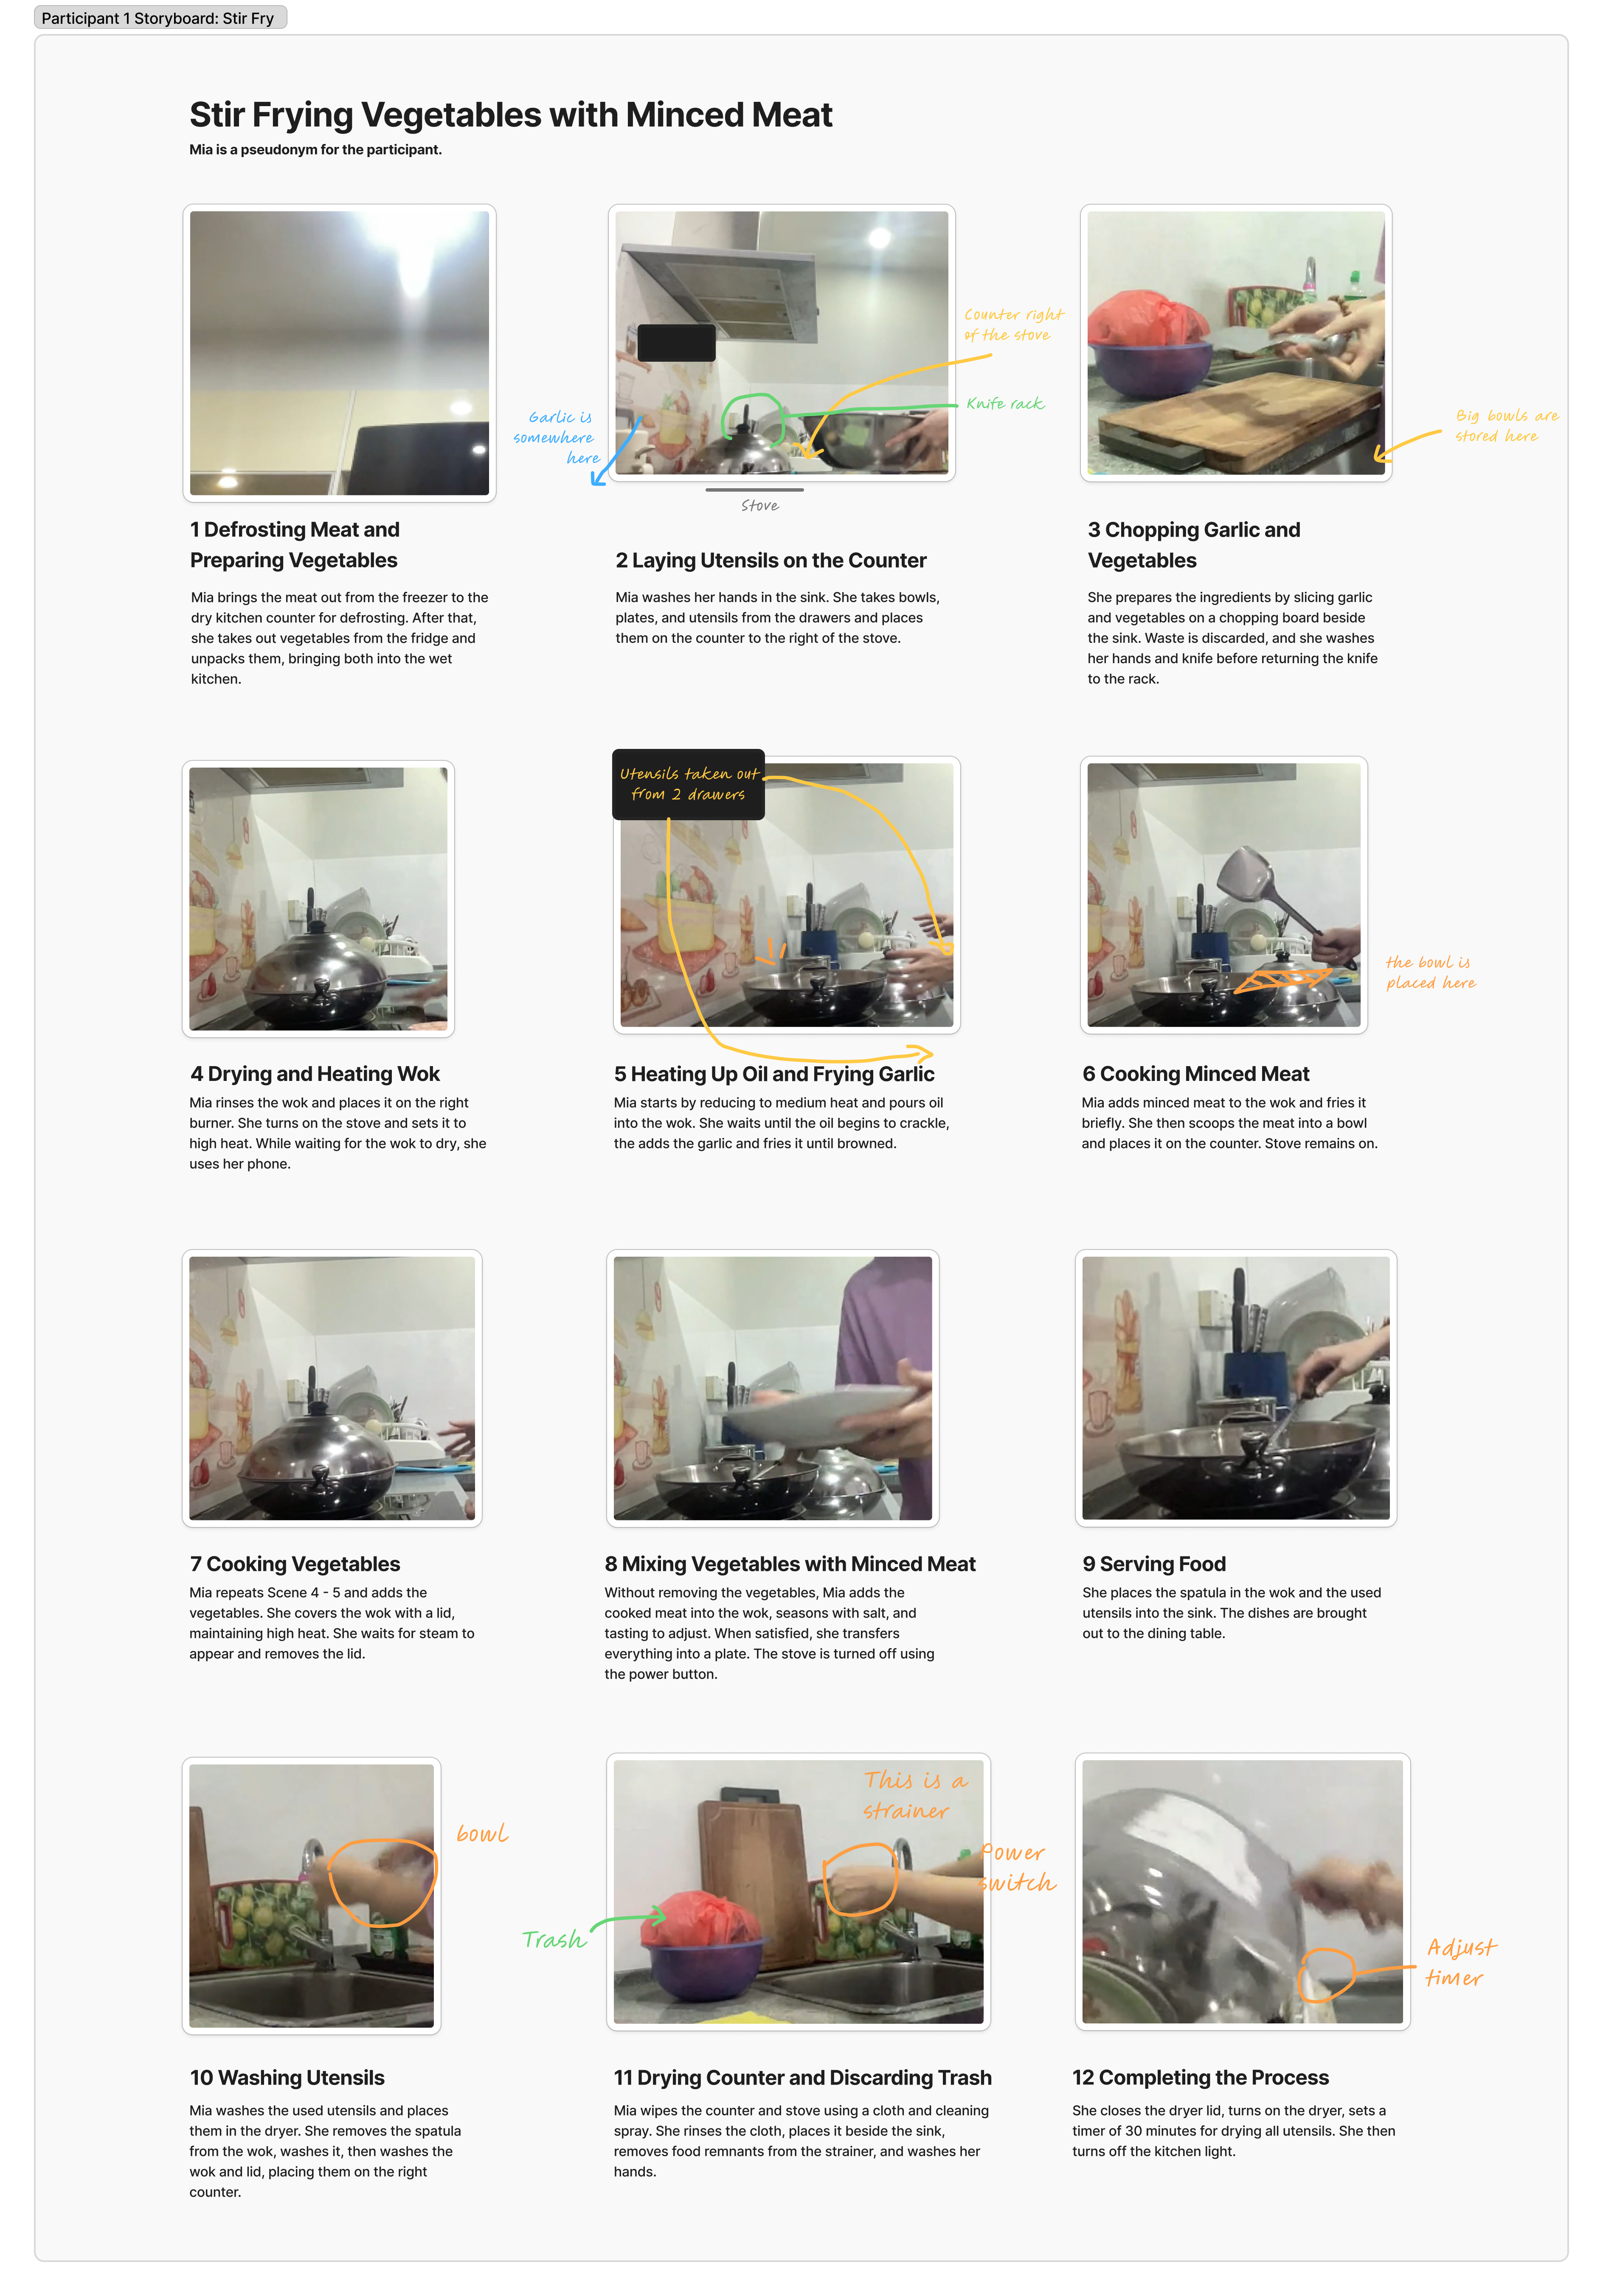
\includegraphics[width=\columnwidth]{figures/p1_storyboard.png}
	\caption{Storyboard for participant 1 illustrating a stir fry cooking process.}
	\label{fig:storyboard_1}
\end{figure}




\end{document}
\endinput
%%
%% End of file `sigconf-main.tex'.